\section{Case Study}
%\section{Exploring Bias Mitigation in ChatGPT through Zero-Shot Prompt Learning with ICQ}
\label{sec:mitigatingbiases}
\begin{figure}[th]
\centering
\includegraphics[width=\columnwidth]{picture/prompt.eps}
\caption{Prompts. }
%\KZ{``Possible distributions of the same feature''}}
\label{fig:prompt}
\end{figure}

Recently, ChatGPT, a large language model (LLM) released by OpenAI, has garnered significant interest 
from the NLP community.
ChatGPT, a GPT-x~\footnote{Currently, x is either 3.5 or 4, and in the subsequent experimental process, the ChatGPT we use is based on GPT-3.5.} series model, 
is trained through Reinforcement Learning from Human Feedback (RLHF)~\cite{christiano2017deep} similarly to InstructGPT~\cite{ouyang2022training}.
In this section, we investigate if zero-shot ChatGPT is influenced by bias features, using a case study focused on the word ``no'' in the MNLI dataset.
We aim to compare the effectiveness of different prompts and select the best one for mitigating bias 
based on a single bias feature. 

\subsection{Dataset}
\label{sec:chatgptdata}
We selected test instances from the MNLI dataset 
to study the influence of the word ``no'' on ChatGPT's performance. 
The original test set has \textit{Contradiction}: 3240, 
\textit{Entailment}: 3463, and \textit{Neutral}: 3129 instances. 
Instances containing ``no'' are distributed as follows: \textit{Contradiction}:229, 
\textit{Entailment}: 38, and \textit{Neutral}: 46.

For the accuracy test, we used all 313 instances 
with ``no'' and an equal number of instances without 
``no'', randomly chosen from the remaining test set. 
This ensures a balanced evaluation of ChatGPT's performance.

For the distribution test, we selected 38 
instances per label containing ``no'', 
resulting in a total of 114 instances. 

\subsection{Prompts}
We have four prompts in~\figref{fig:prompt}:
The first prompt is proposed by ChatGPT itself. 
We ask, ``What is the best prompt for the MNLI task according to you?''. 
ChatGPT returns prompt 1 for us. 
The second prompt is inspired by previous work~\cite{qin2023chatgpt}.
The third and fourth prompts are created by adding ``Let's think step by step''~\cite{kojima2022large}
to prompt 1 and prompt 2 with the ``chain of thought'' (CoT) thinking, respectively. 
This modification has been shown to significantly improve 
the performance of InstructGPT on reasoning tasks~\cite{ouyang2022training}.

\subsection{ICQ Results}
\label{sec:chatgptacc}
\begin{figure}[th]
\centering
\begin{minipage}{0.45\linewidth}
\centering
\scriptsize
\begin{tabular}{c|ccc}
\toprule
\textbf{Prompt} & Acc (``no'') & Acc (w/o ``no'') & $\Delta Acc$ \\ \midrule
P1  & 74.34& 77.32& -2.98   \\ \hline
P2&  75.42& 74.18 & 1.24 \\ \hline
P1 + CoT  & 78.35& 77.28&1.07  \\ \hline
P2 + CoT&  76.67& 76.40&  0.27 \\ \hline
 \bottomrule
\end{tabular}
\caption{Accuracy test results (\%). P1=Prompt 1, P2=Prompt 2.}
\label{tab:accuracy}
\end{minipage}
\hfill
\begin{minipage}{0.4\linewidth}


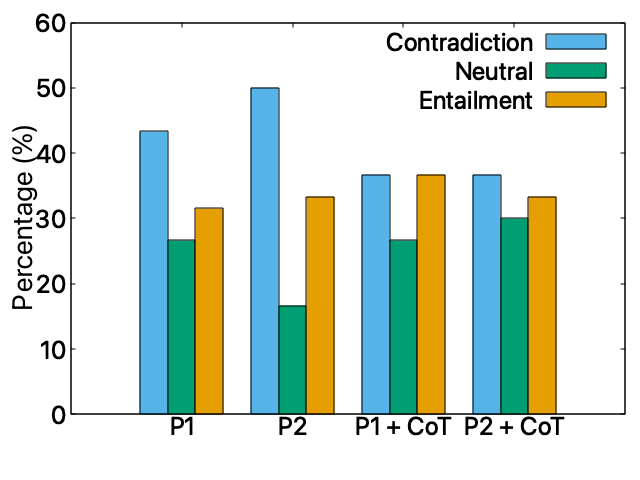
\includegraphics[width=\columnwidth]{data/cue.png}
\caption{Distribution test results. }
\label{fig:cue_chatgpt}


\end{minipage}
\end{figure}


We evaluated the model's accuracy using different prompts on instances 
with and without the word ``no.'' The results are shown in~\tabref{tab:accuracy}. 
P1 demonstrates a negative $\Delta$ Acc, 
indicating difficulty in generalizing when ``no'' is present. 
P2 exhibits a positive $\Delta$ Acc, suggesting better generalization. 
Adding ``CoT'' to both prompts reduces bias risk. 
P1 + CoT shows the most significant improvement in 
Acc (``no''), but P2 + CoT has the smallest absolute 
$\Delta$ Acc, indicating the least sensitivity to ``no'' 
and the lowest bias risk among the tested prompts.

Besides, we analyzed the model's prediction distribution~\figref{fig:cue_chatgpt} 
for the different prompts on the stress test set 
containing the word ``no'' with balanced label distribution. 
Distribution test results reveal imbalances in P1 and P2 
prediction distributions, with P1 and P2 leaning towards 
predicting contradictions. Adding ``CoT'' mitigates these imbalances, 
leading to more balanced distributions. 
P2 + CoT presents the most balanced distribution 
among the labels, supporting its lowest bias risk.

In conclusion, 
our case study demonstrates that zero-shot 
ChatGPT can be influenced by bias features, and the 
choice of prompt can have a substantial effect on its performance.
By comparing the effectiveness of different prompts, 
P2 + CoT exhibits the lowest bias risk based on both tests. 
The ``CoT'' strategy is effective in reducing bias risk. 
These findings suggest that ChatGPT's self-recommended prompt 
(P1) may not always be optimal, emphasizing the importance of 
human intervention and continuous exploration to optimize performance and reduce bias risks. 

\subsection{Discussion and Future Work}
\label{sec:discussion}

Our study has taken important initial steps in model evaluation 
and exploration by providing a lightweight yet effective 
method to reveal statistical biases and cues in NLU datasets. However, further research is needed to obtain a comprehensive understanding of model behavior and address remaining questions.

First, 
we need to extend our focus beyond the MNLI dataset's 
``no'' feature to other features and tasks in order 
to generalize our findings and deepen our understanding of prompt design and bias mitigation.

Second, determining the best approach for optimizing models and selecting prompts 
when dealing with multiple features is a crucial issue that 
will guide our next steps in scientific research.

Third, as the impact of prompts varies across tasks and domains, 
future research should involve extensive prompt exploration and testing for specific applications.

%Additionally, the effectiveness and generalizability of the ``CoT'' 
%strategy in different settings and language models remain open questions, which we will address in future work.

By tackling these challenges, we aim to develop more 
reliable, robust, and unbiased AI systems through comprehensive model evaluation and bias mitigation research.


